\section{Auswertung}
\label{sec:Auswertung}

\subsection{Wheatston'sche Brückeschaltung}
Mit Hilfe der Wheatston'schen Brückenschaltung werden zwei unbekannte Wiederstände $R_{13}$ = Wert13 und $R_{14}$ = Wert14 bestimmt. Dies geschieht mit Formel \ref{eqn:R_x}, die Werte und Ergebnisse sind in den Tabellen \ref{tab:Wheat1} und \ref{tab:Wheat2} aufgeführt. $\overline{R_\text{13,14}}$ entspricht hierbei den gemittelten Werten für die gesuchten Widerstände. Der Wert $R_2$ hat eine Toleranz von 0.2\% und $\frac{R_3}{R_4}$ hat eine Toleranz von 0.5\%.

\begin{table}[H] %R13
  \centering
  \begin{tabular}{c c c c c}
    \toprule
    $R_2$ / $\Omega$ & $R_3$ / $\Omega$ & $R_4$ / $\Omega$ & $R_{13}$ / $\Omega$ & $\overline{R_{13}}$ / $\Omega$ \\
    \midrule
    332 & 735 & 265 & \num{322.8 +- 1.7} &  \\
    500 & 648 & 352 & \num{321.0 +- 1.7} &  \num{326.6 +- 1.0}\\
    664 & 582 & 418 & \num{336.0 +- 1.8} &  \\
  \end{tabular}
  \caption{Werte für die Bestimmung von $R_{13}$.}
  \label{tab:Wheat1}
\end{table}

\begin{table}[H] %R14
  \centering
  \begin{tabular}{c c c c c}
    \toprule
    $R_2$ / $\Omega$ & $R_3$ / $\Omega$ & $R_4$ / $\Omega$ & $R_{14}$ / $\Omega$ & $\overline{R_{14}}$ / $\Omega$ \\
    \midrule
    332 & 493 & 507 & \num{920.8 +- 5.0} &  \\
    500 & 391 & 609 & \num{920.5 +- 5.0} &  \num{921.9 +- 2.9}\\
    664 & 336 & 664 & \num{924.5 +- 5.0} &  \\
  \end{tabular}
  \caption{Werte für die Bestimmung von $R_{14}$.}
  \label{tab:Wheat2}
\end{table}

\subsection{Kapazitätsmessbrücke}
Mit Hilfe der Kapazitätsmessbrücke werden zwei unbekannte verlustfreie Kapazitäten \\ $C_2$ = Wert2 und $C_3$ = Wert3 und eine verlustbehaftete Kapazität $C_8$ = Wert8 bestimmt. Dies geschieht mit Formel \ref{eqn:R_x} für $C_2$, $C_3$ und mit den Formeln \ref{eqn:R_x}, \ref{eqn:C_x} für $C_8$ und $R_8$. Die Messwerte und Ergebnisse sind in den Tabellen \ref{tab:Kapa1} bis \ref{tab:Kapa3} aufgeführt. $\overline{C_\text{2,3,8}}$ entspricht hierbei den gemittelten Werten für die gesuchten Kapazitäten.
Der Wert $C_2$ hat eine Toleranz von 0.2\% und $\frac{R_3}{R_4}$ hat eine Toleranz von 0.5\%, allerdings hat $R_2$ nun eine Toleranz von 3\%.

\begin{table}[H] %C2
  \centering
  \begin{tabular}{c c c c c}
    \toprule
    $C_2$ / nF & $R_3$ / $\Omega$ & $R_4$ / $\Omega$ & $C_2$ / $\mu$F & $\overline{C_2}$ / $\mu$F \\
    \midrule
    597 & 285 & 715 & \num{1.498 +- 0.008} &  \\
    750 & 329 & 671 & \num{1.530 +- 0.008} &  \num{1.517 +- 0.005}  \\
    994 & 395 & 605 & \num{1.522 +- 0.008} &  \\
  \end{tabular}
  \caption{Werte für die Bestimmung von $C_2$.}
  \label{tab:Kapa1}
\end{table}

\begin{table}[H] %C3
  \centering
  \begin{tabular}{c c c c c}
    \toprule
    $C_2$ / nF & $R_3$ / $\Omega$ & $R_4$ / $\Omega$ & $C_3$ / $\mu$F & $\overline{C_3}$ / $\mu$F \\
    \midrule
    597 & 593 & 607 & \num{40.97 +- 0.22} &  \\
    750 & 639 & 361 & \num{42.37 +- 0.23} &  \num{41.65 +- 0.13}  \\
    994 & 705 & 295 & \num{41.59 +- 0.22} &  \\
  \end{tabular}
  \caption{Werte für die Bestimmung von $C_3$.}
  \label{tab:Kapa2}
\end{table}

\begin{table}[H] %C8 R8
  \centering
  \begin{tabular}{c c c c c c c c}
    \toprule
    $C_2$ / nF & $R_2$ / $\Omega$ & $R_3$ / $\Omega$ & $R_4$ / $\Omega$ & $C_8$ / $\mu$F & $R_8$ / $\Omega$ & $\overline{C_8}$ / $\mu$F & $\overline{R_8}$ / $\Omega$ \\
    \midrule
    597 & 304 & 671 & 329 & \num{29.27 +- 0.16} & \num{149.1 +- 4.5} & & \\
    750 & 228 & 722 & 278 & \num{28.88 +- 0.16} & \num{87.8 +- 2.7} & \num{29.11 +- 0.09} & \num{96.5 +- 1.8} \\
    994 & 179 & 773 & 227 & \num{29.19 +- 0.16} & \num{52.6 +- 1.6} & & \\
  \end{tabular}
  \caption{Werte für die Bestimmung von $C_8$ und $R_8$.}
  \label{tab:Kapa3}
\end{table}

\newpage
\subsection{Induktivitätsmessbrücke}
\label{sec:Induk}
Mit Hilfe der Induktivitätsmessbrücke wird die verlustbehaftete Induktivität $L_{19}, R_{19}$ = Wert19 einer unbekannten Spule bestimmt. Dies geschieht mit den Formeln \ref{eqn:R_x} und \ref{eqn:L_x}. Die Messwerte und Ergebnisse sind in der Tabelle \ref{tab:Induk1} aufgeführt. Die baubedingten Fehler von $R_2$ und $\frac{R_3}{R_4}$ sind die gleichen wie im vorangegangenen Kapitel, der Fehler von$L_2$ beträgt 0.2\%.

\begin{table}[H] %L19 R19
  \centering
  \begin{tabular}{c c c c c c c c}
    \toprule
    $L_2$ / mH & $R_2$ / $\Omega$ & $R_3$ / $\Omega$ & $R_4$ / $\Omega$ & $L_{19}$ / mH & $R_{19}$ / $\Omega$ & $\overline{L_{19}}$ / mH & $\overline{R_{19}}$ / $\Omega$ \\
    \midrule
    14.6 & 286 & 281 & 719 & \num{5.706 +- 0.029} & \num{111.8 +- 0.6} & & \\
    20.1 & 287 & 287 & 713 & \num{8.090 +- 0.040} & \num{115.5 +- 0.6} & \num{6.898 +- 0.025} & \num{113.6 +- 0.4} \\
  \end{tabular}
  \caption{Werte für die Bestimmung von $L_{19}$ und $R_{19}$.}
  \label{tab:Induk1}
\end{table}

\subsection{Maxwell-Brücke}
\label{sec:Maxwell}
Mit Hilfe der Maxwell-Brücke soll die gleiche Spule untersucht werden welche auch für die Induktivitätsmessbrücke verwendet wurde, dadurch erhält man einen vergleichbaren Wert. Die verwendete Kapazität $C_4$ = 750 nF bleibt für die gesamte Messung unverändert. Durch einsetzen in die Formeln \ref{eqn:R_x}, \ref{eqn:L_m} erhält man $L_{19}$ und $R_{19}$. Die Messwerte und Ergebnisse sind in Tabelle \ref{tab:Induk2} aufgelistet.

\begin{table}[H] %L19 R19
  \centering
  \begin{tabular}{c c c c c c c}
    \toprule
    $R_2$ / $\Omega$ & $R_3$ / $\Omega$ & $R_4$ / $\Omega$ & $L_{19}$ / mH & $R_{19}$ / $\Omega$ & $\overline{L_{19}}$ / mH & $\overline{R_{19}}$ / $\Omega$ \\
    \midrule
    332 & 215 & 655 & \num{53.5 +- 1.6} & \num{109.0 +- 4.6} & & \\
    664 & 95 & 538 & \num{47.3 +- 1.4} & \num{117.2 +- 5.0} & \num{57.6 +- 1.0} & \num{115.6 +- 2.8} \\
    1000 & 96 & 796 & \num{72.0 +- 2.2} & \num{120.6 +- 5.1} & & \\
  \end{tabular}
  \caption{Werte für die Bestimmung von $L_{19}$ und $R_{19}$.}
  \label{tab:Induk2}
\end{table}

\newpage
\subsection{TT-Brücke}
Wie man in der Tabelle \ref{tab:TT-Brucke} erkennen kann, wird die Brückenspannung bei ca. 380 Hz minimal und beträgt in etwa 0.02 V. \\
Der theoretische minimal Wert lässt sich mit folgender Formel berechnen:
\begin{align*}
  f_{0,\text{theo}} & = \frac{1}{RC} = (\num{382.1 +- 1.2}) \, \text{Hz} \\
  R & = 1000 \, \Omega \\
  C & = (\num{4.165 +- 0.013}) \cdot 10^{-7} \, \text{F}.
\end{align*}

\begin{table}[H] %f gegen U
  \centering
  \begin{tabular}{c c}
    \toprule
    f / Hz & $U_\text{br}$ / V \\
    \midrule
      20	  &  4.56  \\
      70	  &  3.76  \\
      180	  &  1.78  \\
      200	  &  1.51  \\
      220	  &  1.28  \\
      240	  &  1.07  \\
      260	  &  0.88  \\
      280	  &  0.70  \\
      300	  &  0.56  \\
      320	  &  0.40  \\
      340	  &  0.26  \\
      360	  &  0.14  \\
      380	  &  0.02  \\
      400	  &  0.21  \\
      420	  &  0.23  \\
      440	  &  0.33  \\
      460	  &  0.43  \\
      480	  &  0.52  \\
      500	  &  0.61  \\
      520	  &  0.70  \\
      540	  &  0.78  \\
      560	  &  0.87  \\
      580	  &  0.96  \\
      700	  &  1.37  \\
      1000	&  2.14  \\
      2000	&  3.26  \\
      7000	&  3.90  \\
      15000	&  3.92  \\
      30000	&  3.92  \\
  \end{tabular}
  \caption{Messwerte der Brückenspannung und der Frequenz von der TT-Brückenschaltung.}
  \label{tab:TT-Brucke}
\end{table}

\begin{figure}[H]
  \centering
  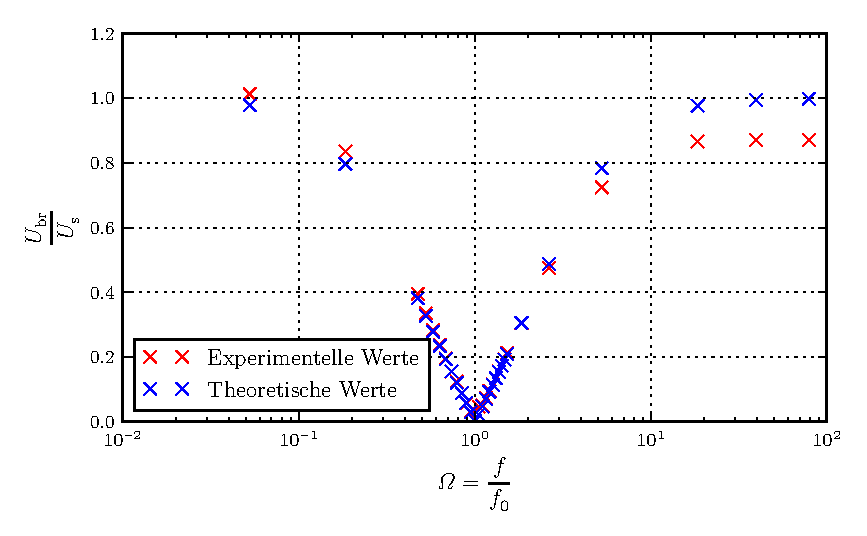
\includegraphics[width=\textwidth]{AufgabeE.pdf}
  \caption{Theoretische und experimentelle Werte der TT-Brückenschaltung.}
  \label{fig:AufgabeE}
\end{figure}

Für die Bestimmung des Klirrfaktors $k$ wird zunächst genähert, dass die Summe der
Oberwellen nur von dem Term der zweiten Oberwelle bestimmt wird. Damit folgt, dass
\begin{align}
  k = & \frac{\sqrt{{U_2}^2 + {U_3}^2 + ...}}{U_1} = \frac{U_2}{U_1}  \\
  U_1 & = 4.5 \, \text{V}    \\
  U_2 & = \frac{U_\text{br}}{f(2)}    \\
      & U_\text{br} = 0.02 \, \text{V}   \\
      & f(2) = \frac{(1 - 2^2)^2}{(1 - 2^2)^2 + 16 \cdot 2^2} = 0.1233  \\
  U_2 & = \frac{0.02 \text{V}}{0.1233} = 0.1622 \, \text{V}  \\
  k = & \frac{0.1622 \text{V}}{4.5 \, \text{V}} = 0.036
\end{align}
ist.








.
